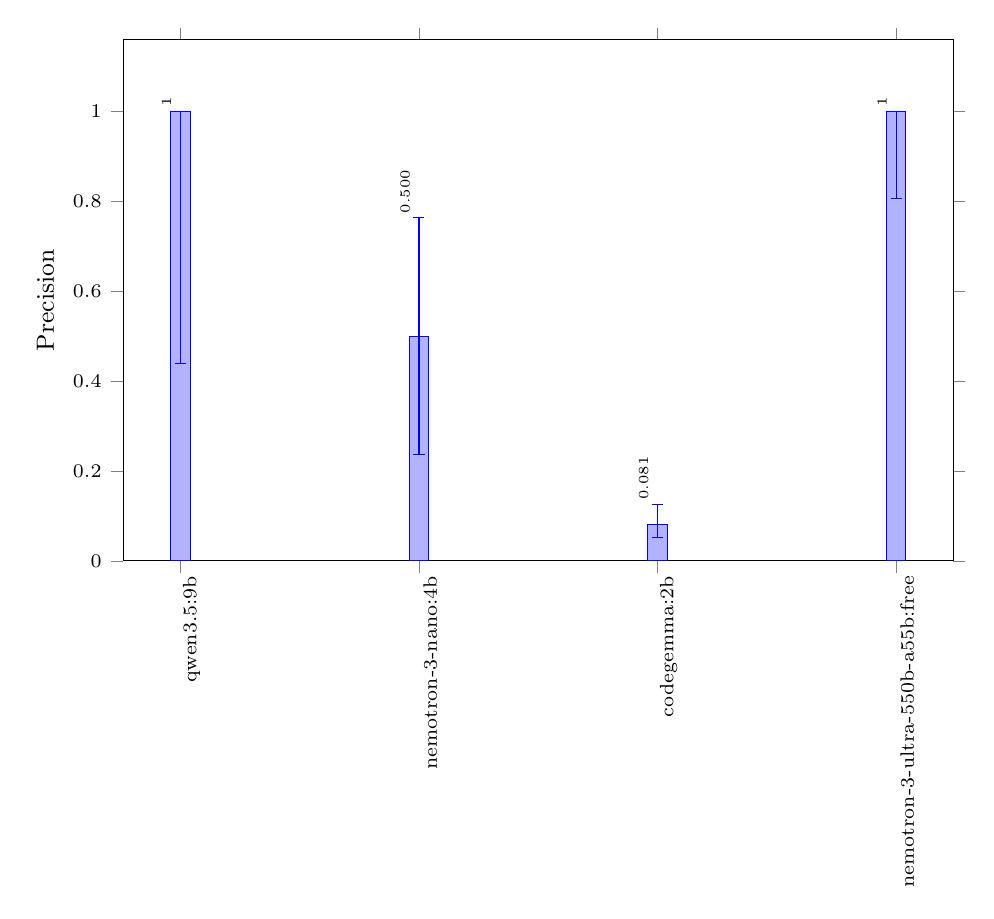
\begin{tikzpicture}
\begin{axis}[
  ybar,
  bar width=7pt,
  bar shift=0pt,
  width=\textwidth,
  height=8.2cm,
  ylabel={Precision},
  xtick={0,1,2,3},
  xticklabels={qwen3.5:9b,nemotron-3-nano:4b,codegemma:2b,nemotron-3-ultra-550b-a55b:free},
  x tick label style={rotate=90, anchor=east, font=\scriptsize, inner sep=1pt, yshift=-4pt},
  y tick label style={font=\scriptsize},
  label style={font=\small},
  ymin=0,
  ymax=1.160000,
  enlarge x limits=0.08,
  tick align=outside,
  clip=false,
]
\addplot+[
  bar shift=0pt,
  error bars/.cd,
  y dir=both,
  y explicit,
  error bar style={thin}
] table[x=x,y=y,y error minus=minus,y error plus=plus] {
x y minus plus
0 1.000000 0.561497 0.000000
1 0.500000 0.263407 0.263407
2 0.080952 0.029797 0.044853
3 1.000000 0.193608 0.000000
};
\addplot[
  only marks,
  mark=none,
  bar shift=0pt,
  forget plot,
  nodes near coords,
  point meta=explicit symbolic,
  every node near coord/.append style={font=\tiny, rotate=90, anchor=west, inner sep=1.5pt, yshift=5pt, fill=white, fill opacity=0.9, text opacity=1},
] table[x=x,y=y,meta=label] {
x y label
0 1.000000 {1}
1 0.763407 {0.500}
2 0.125805 {0.081}
3 1.000000 {1}
};
\end{axis}
\end{tikzpicture}
